\documentclass[10pt]{article}
%\documentclass[10pt,twocolumn]{article}
%\documentclass[12pt]{article}
%\pagestyle{plain}

\special{papersize=8.5in,11in}

% load graphics packages and allow conversion of certain image types
\usepackage{geometry} 
\geometry{letterpaper} 
\geometry{margin=1in}
\usepackage[parfill]{parskip}    % Activate to begin paragraphs with an empty line
\usepackage{graphicx}
\usepackage{amssymb, amsmath} % math commands
\usepackage{epstopdf}
\usepackage{fancyhdr}
\usepackage{mathrsfs}
\usepackage{accents}
\usepackage{bm} % math commands
\DeclareGraphicsRule{.tif}{png}{.png}{`convert #1 `basename #1 .tif`.png}
\usepackage{subfigure} % do multiple figures next to each other
\usepackage{hyperref}   % use for hypertext links, including those to external documents and URLs

%%%%%%%%%%%%%%%%%%%%%%%%%%%%%%%%%%%%%%%%%%%%
% Format code
%%%%%%%%%%%%%%%%%%%%%%%%%%%%%%%%%%%%%%%%%%%%
\usepackage{listings} 
\usepackage[usenames,dvipsnames]{color}
\lstset{ %
language=C++,                % the language of the code
commentstyle=\color{Green},
basicstyle=\footnotesize,       % the size of the fonts that are used for the code
keywordstyle=\color{Red}\bfseries,
stringstyle=\color{Purple}\bfseries,
%basicstyle=\tiny,
numbers=left,                   % where to put the line-numbers
numberstyle=\footnotesize,      % the size of the fonts that are used for the line-numbers
stepnumber=5,                   % the step between two line-numbers. If it's 1, each line 
                                % will be numbered
numbersep=5pt,                  % how far the line-numbers are from the code
%backgroundcolor=\color{white},  % choose the background color. You must add \usepackage{color}
showspaces=false,               % show spaces adding particular underscores
showstringspaces=false,         % underline spaces within strings
showtabs=false,                 % show tabs within strings adding particular underscores
%frame=single,                   % adds a frame around the code
frame=left,
tabsize=2,                      % sets default tabsize to 2 spaces
captionpos=b,                   % sets the caption-position to bottom
breaklines=true,                % sets automatic line breaking
breakatwhitespace=false,        % sets if automatic breaks should only happen at whitespace
title=\lstname,                 % show the filename of files included with \lstinputlisting;
                                % also try caption instead of title
%escapeinside={\%*}{*)},         % if you want to add a comment within your code
%morekeywords={*,...}            % if you want to add more keywords to the set
}
%%%%%%%%%%%%%%%%%%%%%%%%%%%%%%%%%%%%%%%%%%%%

%\usepackage[sectionbib]{natbib}
\usepackage[sectionbib]{chapterbib}

% these are commands i made
\newcommand{\sm}[1]{\mbox{\unboldmath{$#1$}}} % not sure of the value of this
\newcommand{\hv}[1]{\underrightarrow{\bm{#1}}} % Hughes' vector
\newcommand{\huv}[1]{\hat{\underrightarrow{\bm{#1}}}} % Hughes' unit vector
\newcommand{\uv}[1]{\hat{\bm{#1}}} % unit vector
\newcommand{\dt}[1]{\frac{d #1}{dt}} % time derivative of a variable
\newcommand{\der}[2]{\frac{d #1}{d #2}} % derivative of a variable wrt another variable
\newcommand{\dpar}[2]{\frac{\partial #1}{\partial #2}} % partial derivative of a variable wrt another variable
\newcommand{\rf}[1]{\bm{\mathscr{#1}}}
\newcommand{\figref}[1]{{\bf Figure \ref{#1}}}
\newcommand{\dmathring}[1]{\accentset{\circ{}\circ{}}{#1}} 
\newtheorem{theorem}{Theorem}[section]
\newtheorem{definition}{Definition}

\pagestyle{headings}

\flushbottom

\title{\textsf{Holonomic Soccer Robot}}

\author{
%\hline 
\begin{minipage}[b]{2in}
	\centering
	
\includegraphics[height=1in]{pics/qrcode.png}
\end{minipage}
%\hspace{0.5cm}
\begin{minipage}[b]{3in}
	Kevin J. Walchko, PhD \\ \\ \\
	%US Air Force \\
	Code: https://github.com/walchko/soccer \\
	Email: \texttt{walchko@verizon.net} 
\end{minipage}
\\
\hline
}

\begin{document}

%\begin{titlepage}

\maketitle

%\end{titlepage}

 
\begin{abstract}
This paper describes the development of a holonomic robot using omni directional wheels. Both a development of the kinematic and dynamical equations of motion are derived and used as a foundation for gaining further insight into the capabilities of the robot. A discussion of the vision system used to detect objects and obstacles during navigation. 
\end{abstract}

\section{Variables}
\begin{table}[h]
	\begin{center}
		\begin{tabular}{ccl}
		\hline
		Parameter & Units & Description \\
		\hline
		%$T$ 	& kg m/s$^2$ 		& kinetic energy \\
		%$V$ & kg m$^2$/s$^2$     & potential energy \\
		$R$ & m & robot radius \\
		%$e$ & V & motor voltage \\
		M & kg & mass of robot \\
		I & $kg \cdot m^2$ & inertia of robot \\
		$I_w$ & kg$\cdot$m$^2$ & inertia of wheel \\
		$a_i$ & m/$sec^2$ & acceleration in the $i^{th}$ direction \\
		$v_i$ & m/sec & velocity in the $i^{th}$ direction \\
		$\omega_i$ & rad/sec & $i^{th}$ wheel speed \\
		$r_w$ &  m & wheel radius \\
		$\tau_i$ & N$\cdot$m & wheel torque \\
		$F_i$ & N & traction force (vector) \\
		$f_i$ & N &  magnitude of traction force ($\|F_i\|$) \\
		\hline
		\end{tabular}
	\end{center}
\end{table}

\section{Introduction}

%\lstinputlisting[language=C++]{filter_test.cpp}

Robots come in a variety of types and configurations: wheeled, tracked, legs, flying, etc. Common wheeled robots typically have two wheels (directly driven) with a caster wheel to make the robot stable. There are some without the caster wheel and employ a control system to keep them upright (inverted pendulum problem) and resemble a Segway scooter. All of these two wheeled robot are non-holonomic systems. 

\begin{definition}
A non-holonomic system in physics and mathematics is a system whose state depends on the path taken to achieve it. An automobile is an example of a non-holonomic vehicle. The vehicle has three degrees of freedom�its position in two axes, and its orientation relative to a fixed heading. Yet it has only two controllable degrees of freedom�acceleration/braking and the angle of the steering wheel�with which to control its position and orientation. \cite{wiki_non_holonomic}
\end{definition}

Due to these constraints, a holonomic robot (\figref{robot}) which could travel in any direction and immediately change its position and orientation is much more desirable. There are a variety of different wheels which make this type of robot possible such as mecanum or omni wheels (\figref{wheel}).

Omni wheels operate like standard wheels in that the force is produced normal to the motor's axis of rotation and as a result of friction (no slip assumption). However, there are a series of smaller wheels which ring the main wheel and allow the wheel to slip in the direction of the motor rotational axis. Note that no force is produced parallel to the motor axis, just slippage.

\section{Holonomic Dynamics}


\begin{figure*}[tb]
	\begin{minipage}[htb]{2.5in}
		\centering
 		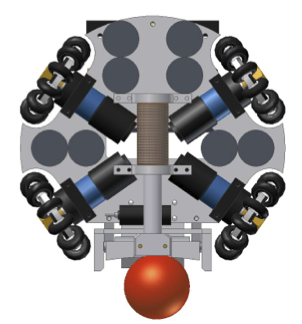
\includegraphics[height=2.5in]{pics/holonomic_robot.png} 
		\caption{\label{robot}Holonomic soccer robot using 4 omni directional wheels and a kicking motor used to hit the red ball into a goal. \cite{Radu1}.}  
 	\end{minipage}
 	\hfill
 	\begin{minipage}[htb]{2.5in}
		\centering
 		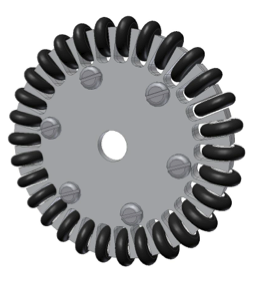
\includegraphics[height =2.5in]{pics/omni_wheel.png} 
		\caption{\label{wheel}Omni directional wheel used on the soccer robot which allows movement in any direction.} 
 	\end{minipage} 
\end{figure*}  


\begin{figure*}[htb]
	%\begin{minipage}[htb]{2.5in}
		\centering
 		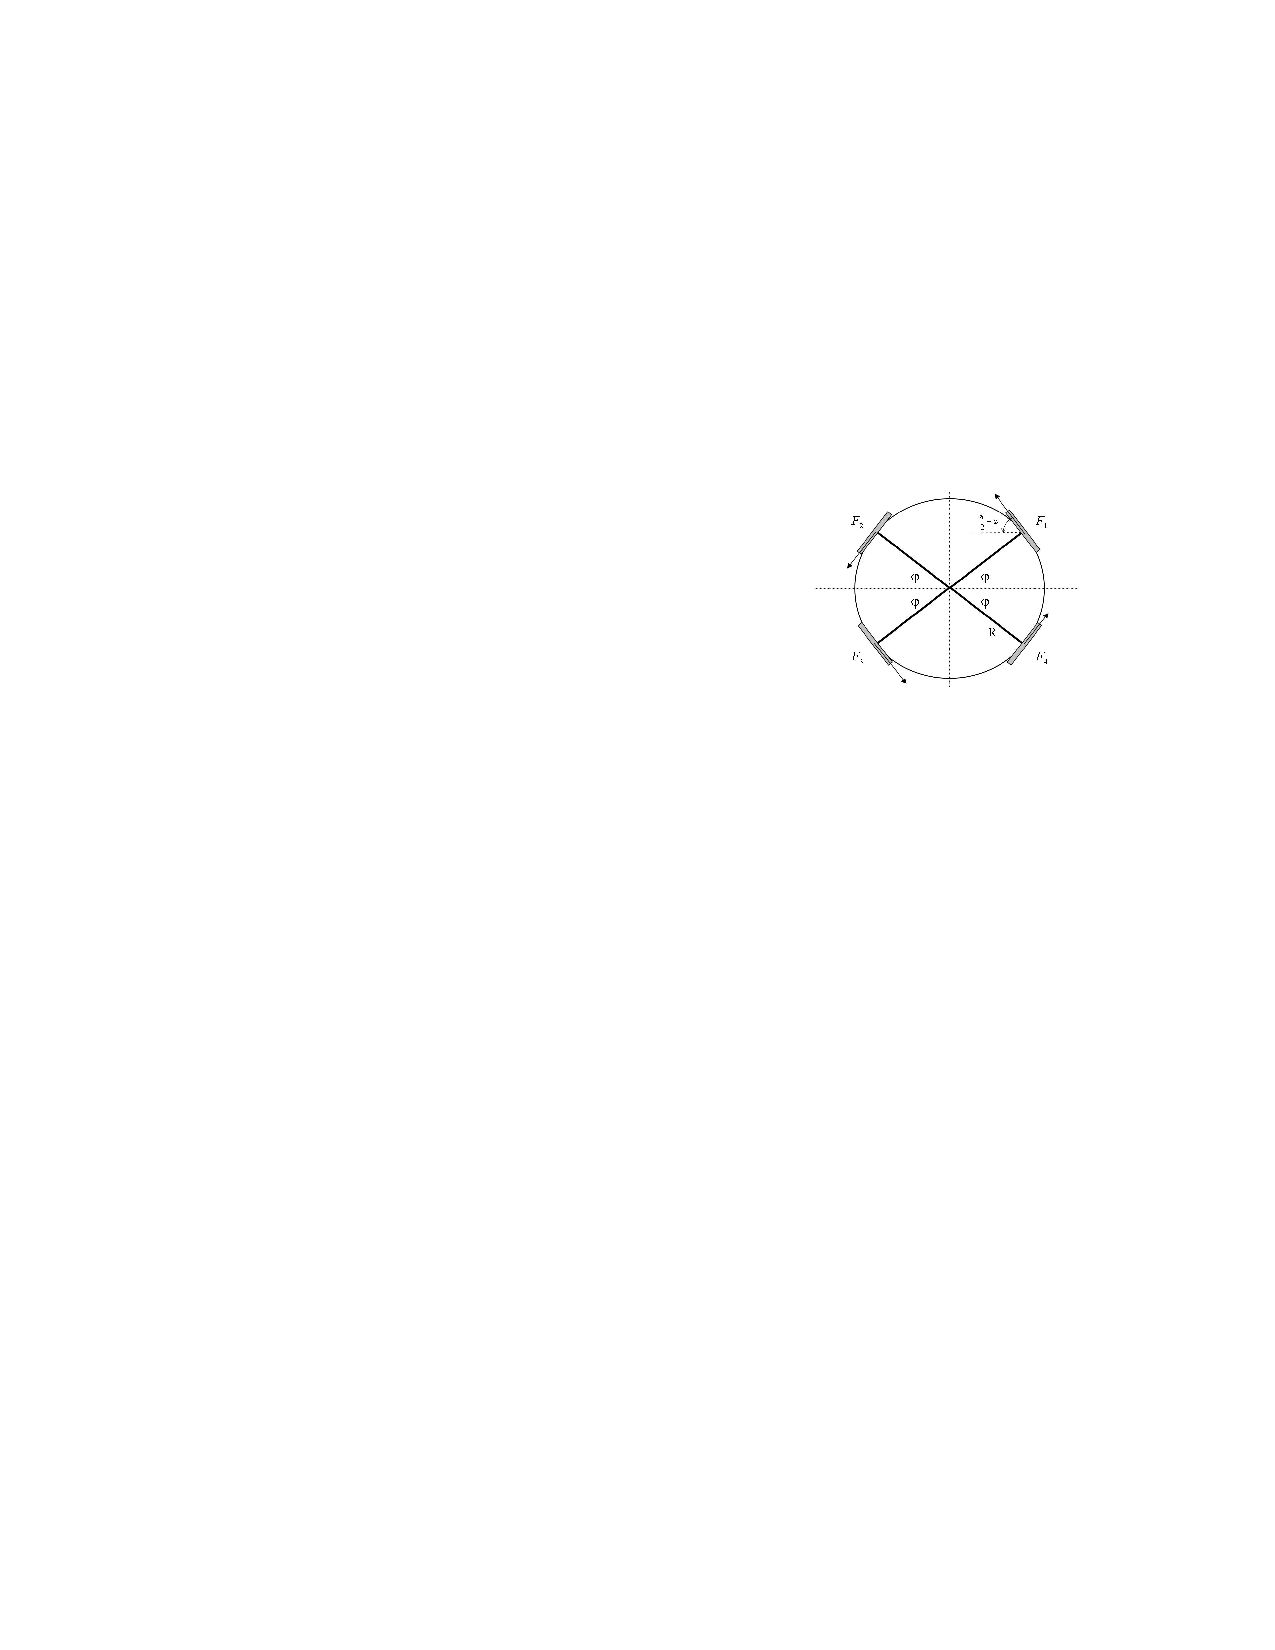
\includegraphics[height=2.5in]{pics/coordinate_system.pdf} 
		\caption{\label{coordinate}Coordinate system tied to the body of the robot with the origin located at the center of mass. Note that the x-axis points straight up and the y-axis points to the right. Also, the motor angle $\phi$ is defined as the angle measured from the y-axis. The forces (F) are the results of the motors spinning in the positive direction according to the right hand rule. Note also that no force is produced parallel to the motor's axis of rotation.}  
 	%\end{minipage}
 	%\hfill
 	%\begin{minipage}[htb]{2.5in}
		%\centering
 		%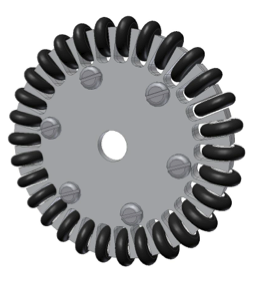
\includegraphics[height =2.5in]{pics/omni_wheel.png} 
		%\caption{\label{wheel}Omni directional wheel which allows movement in any direction.} 
 	%\end{minipage} 
\end{figure*}  


The dynamics for a holonomic robot, such as \figref{robot}, with 4 omni directional wheels (see \figref{wheel}, can be derived using Euler-Largrange ($\mathcal{L}$) which defines a system's kinectic ($T$) and potential ($V$) energies in relation to a set of generalized coordinates ($q$) and generalized forces ($Q$):

\begin{eqnarray}
	\mathcal{L}=T-V \\
	\frac{d}{dt} \left\{ \dpar{ \mathcal{L} }{\dot q} \right\} - \dpar{ \mathcal{L} }{q} = Q \\
	T = \frac{1}{2}M(\dot x^2 + \dot y^2)+ \frac{1}{2}J \dot \psi^2 + \frac{1}{2} J_w (\dot \theta_1^2 + \dot \theta_2^2 + \dot \theta_3^2 + \dot \theta_4^2) \\
	V = 0
\end{eqnarray}

\begin{eqnarray}
	F_x = M \ddot x \hspace{1in} F_y = M \ddot y \\
	\tau = J_R \dot \psi \\
	\tau_w = J_w \ddot \theta_1 \hspace{1cm}
	\tau_w = J_w \ddot \theta_2 \hspace{1cm}
	\tau_w = J_w \ddot \theta_3 \hspace{1cm}
	\tau_w = J_w \ddot \theta_4 \\
\end{eqnarray}

where the generalized forces ($Q$) are defined as:

\begin{eqnarray*}
	Q = F \\
	 = 3 \\
\end{eqnarray*}



\begin{eqnarray}
	a=\sum \limits_{i=0}^4 \frac{F_i}{M_i}=\frac{1}{M}(F_1+F_2+F_3+F_4) \label{one} \\
	\dot{\omega}= \sum \limits_{i=0}^4 \frac{\tau_i}{J_R}=\frac{R}{J_R}(f_i+f_2+f_3+f_4)  where \tau_i=Rf_i
\end{eqnarray}

Now looking at figure \ref{coordinate}, and breaking equation \ref{one} up into its x and y components

\begin{eqnarray}
	a_x=\frac{1}{M}(-f_1 \sin(\phi) - f_2 \sin(\phi) + f_3 \sin(\phi) + f_4 \sin(\phi))  \label{two} \\
	a_y=\frac{1}{M}(f_1 \cos(\phi) - f_2 \cos(\phi) - f_3 \cos(\phi) + f_4 \cos(\phi)) \label{three} \\
	\dot{\omega}=\frac{R}{J_R}(f_1+f_2+f_3+f_4) \label{four}
\end{eqnarray}

Now combining these into a matirx.

\begin{eqnarray}
\begin{bmatrix}
	a_x \\
	a_y \\
	\dot \omega
\end{bmatrix} = 
\begin{bmatrix}
	\frac{1}{M} & 0 & 0 \\
	0 & \frac{1}{M} & 0 \\
	0 & 0 & \frac{1}{J_R}
\end{bmatrix}
\begin{bmatrix}
	\sin(\phi) & 0 & 0 \\
	0 & \cos(\phi) & 0 \\
	0 & 0 & 1
\end{bmatrix}
\begin{bmatrix}
	-1 & -1 & 1 & 1\\
	1 & -1 & -1 & 1\\
	1 & 1 & 1& 1
\end{bmatrix}
\begin{bmatrix}
	f_1 \\
	f_2 \\
	f_3 \\
	f_4
\end{bmatrix} \\
\begin{bmatrix}
	a_x \\
	a_y \\
	\dot \omega
\end{bmatrix} = \beta \left[ \phi \right]  \gamma \left[ f_i \right] 
\end{eqnarray}


where $\phi$ is the angle of the motors as defined in \figref{coordinate}, $f_i$ is the magnitude of the force produced by the motors, and $R$ is the radius of the robot. This can be simplified into the following:

\begin{equation}
	P = \frac{1}{M} A(\phi) C F
\end{equation}

where $P$ is the vector of accelerations,  $A(\phi)$ is the matrix which defines the orientation of the motors, $C$ defines the coupling of the motor forces, and $F$ is the vector of forces produced by the motors. The individual motor forces can further be expressed as:

\begin{eqnarray}
	f_i = \frac{\tau_i}{r_w} \\
	F = \frac{1}{r_w} \begin{bmatrix} \tau_1 \\  \tau_2 \\  \tau_3 \\  \tau_4 \end{bmatrix} = \frac{1}{r_w}T
\end{eqnarray}

where $\tau_i$ is the torque produced by the $i^{th}$ motor and $r_w$ is the radius of the wheel. Here we are assuming that all wheels have the same radius $r_w$.

\begin{equation}
	P = \frac{1}{M r_w} A(\phi) C T
\end{equation}

For a given motor orientation (e.g., $\phi$ = 45$^\circ$) this equations provides the acceleration states as a function of motor velocity. However, the reverse would be more useful. Meaning, given a desired set of states, what are the motor velocities required?

\begin{equation}
	T = M r_w pinv(C)A(\phi)^{-1} P
\end{equation}

where

\begin{eqnarray}
	A(\phi)^{-1} = 
	\begin{bmatrix}
		\frac{1}{\sin(\phi)} & 0 & 0 \\
		0 & \frac{1}{\cos(\phi)} & 0 \\
		0 & 0 & \frac{1}{2}
	\end{bmatrix} \\
	pinv(C) = \frac{1}{4}
	\begin{bmatrix}
		-1 & 1 & 1 \\
		-1 & -1 & 1 \\
		1 & -1 & 1 \\
		1 & 1 & 1
	\end{bmatrix}	
\end{eqnarray}

where $pinv()$\footnote[1]{Pseudoinverse: for $m > n$: $A_{left}^{-1}=(A^TA)^{-1}A^T$ or $m < n$: $A_{right}^{-1}=A^T(AA^T)^{-1}$ such that $AA^{-1}=I$ or $A^{-1}A=I$} is defined as the pseudoinverse since $A(\phi)$ is not a square matrix. Finally, substituting these into the original equation, we can calculate the torques given the desired accelerations. 

\begin{equation}
	\begin{bmatrix} \tau_1 \\  \tau_2 \\  \tau_3 \\  \tau_4 \end{bmatrix} = \frac {M r_w} {4}
	\begin{bmatrix}
		-1 & 1 & 1 \\
		-1 & -1 & 1 \\
		1 & -1 & 1 \\
		1 & 1 & 1
	\end{bmatrix}	
	\begin{bmatrix}
		\frac{1}{\sin(\phi)} & 0 & 0 \\
		0 & \frac{1}{\cos(\phi)} & 0 \\
		0 & 0 & \frac{1}{2}
	\end{bmatrix}
	\begin{bmatrix}
		a_x \\
		a_y \\
		R \dot \omega
	\end{bmatrix}
\end{equation}

Now looking at this equation, we notice that $\phi$ can not be equal to 0, 90, 180, 270, or 360 otherwise we get a singularity in the $A(\phi)$ matrix. This however is not an issue in the real world, since the motors would occupy the same physical space and the robot would essentially only have 2 and not 4 motors.

\subsection{State Space}

Now rearranging equations \eqref{two}, \eqref{three}, and \eqref{four} into a state space representation where the state vector is $X = \begin{bmatrix} x & y & R \theta & v_x & v_y & R \omega \end{bmatrix}^T$ and its derivative is $\dot X = \begin{bmatrix} v_x & v_y & R \omega & a_x & a_y & R \dot \omega \end{bmatrix}^T$, the standard formulation is:

\begin{eqnarray}
	\dot X = A X + B u \\
	Y = CX 
\end{eqnarray}

where $A$ is the state transition matrix, $B$ is the input matrix, $u$ is the control input to the system, $C$ is the output matrix which determines which states are visible, and $Y$ is the output vector which is the observable states. Again, the nice thing about formulating the state vector $X$ this way is that all of the units for position are in meters and all of the velocity units are in m/sec.

\begin{eqnarray}
	%X = \begin{bmatrix} x & y & R \theta & v_x & v_y & R \omega \end{bmatrix}^T \\
	%\dot X = \begin{bmatrix} v_x & v_y & R \omega & a_x & a_y & R \dot \omega \end{bmatrix}^T \\
	A = \begin{bmatrix}
		0_{3x3} & I_{3x3} \\
		0_{3x3} & 0_{3x3}
	\end{bmatrix} \\
	B = \frac{1}{M r_w}\begin{bmatrix}
		& 0_{3x4} & \\
		-\sin(\phi) & -\sin(\phi) & \sin(\phi) & \sin(\phi) \\
		\cos(\phi) & -\cos(\phi) & -\cos(\phi) & \cos(\phi) \\
		2 & 2 & 2 & 2 
	\end{bmatrix} \\
	u = \begin{bmatrix} \tau_1 &  \tau_2 &  \tau_3 &  \tau_4 \end{bmatrix}^T \\
	C = \begin{bmatrix} 0 & 0 & 1 & 0 & 0 & 0\\ 0 & 0 & 0 & 0 & 0 & 1 \end{bmatrix}
\end{eqnarray}

The only directly measurable states come from the compass ($\theta$) and the gyro ($\omega$) on the IMU. Position and velocity are not directly measured. Acceleration is also measurable from the IMU and can be used to estimate the velocity and position. 

\begin{eqnarray}
	\dot M X = A X + B u \\
	\begin{bmatrix} v_x \\ v_y \\ R \omega \\ a_x \\ a_y \\ R \dot \omega \end{bmatrix} =
	\begin{bmatrix}
		0_{3x3} & I_{3x3} \\
		0_{3x3} & 0_{3x3}
	\end{bmatrix} 
	\begin{bmatrix} x \\ y \\ R \theta \\ v_x \\ v_y \\ R \omega \end{bmatrix} +
	\frac{1}{M r_w}\begin{bmatrix}
		& 0_{3x4} & \\
		-\sin(\phi) & -\sin(\phi) & \sin(\phi) & \sin(\phi) \\
		\cos(\phi) & -\cos(\phi) & -\cos(\phi) & \cos(\phi) \\
		2 & 2 & 2 & 2 
	\end{bmatrix} 
	\begin{bmatrix} \tau_1 \\  \tau_2 \\  \tau_3 \\  \tau_4 \end{bmatrix}
\end{eqnarray}

Now using this we can show that this system is controllable but not fully observable.

\begin{eqnarray}
	rank \left( \begin{bmatrix} B & AB & A^2B & ... & A^5B \end{bmatrix} \right) = 6 \\
	rank \left( \begin{bmatrix} C \\ CA \\ \vdots \\ CA^5 \end{bmatrix} \right) = 2
\end{eqnarray}

An estimator must be developed in order to properly control the system and keep it stable.

\section{Holonomic Robot Kinematics}

Now performing a similar exercise for what was done with the dynamics, looking at \figref{coordinate}, the velocity of motor 1is given by $v_1 = -\sin(\phi) v_x + \cos(\phi) v_y + R \omega$. Performing this for each wheel gives:

\begin{equation}
	\begin{bmatrix}
		v_1 \\
		v_2 \\
		v_3 \\
		v_4
	\end{bmatrix} = 
	\begin{bmatrix}
		-\sin(\phi)  & \cos(\phi) & 1 \\
		-\sin(\phi) & -\cos(\phi) & 1 \\
		 \sin(\phi) & -\cos(\phi) & 1 \\
		 \sin(\phi)  & \cos(\phi) & 1 
	\end{bmatrix}
	\begin{bmatrix}
		v_x \\
		v_y \\
		R \omega
	\end{bmatrix} = 
	\begin{bmatrix}
		-1 & 1 & 1 \\
		-1 & -1 & 1 \\
		1 & -1 & 1 \\
		1 & 1 & 1
	\end{bmatrix}	
	\begin{bmatrix}
		\sin(\phi) & 0 & 0 \\
		0 & \cos(\phi) & 0 \\
		0 & 0 & 1
	\end{bmatrix}
	\begin{bmatrix}
		v_x \\
		v_y \\
		R \omega
	\end{bmatrix}
\end{equation}

Now setting $\omega$ to zero and calculating only linear movement, we can determine the number of equivalent motors as shown in \figref{fig:equivalent_motors}. For example, setting $\phi$ to 30$^\circ$ (the red line in \figref{fig:equivalent_motors}) and traveling in the x direction only ($ \begin{bmatrix} v_x & v_y & R \omega \end{bmatrix}^T = \begin{bmatrix}1& 0 & 0 \end{bmatrix}^T$), the above equation simplifies to $4 \sin(30)$ or 2 equivalent motors. Repeating for the y direction results in $4 \cos(30)$ or 3.46 equivalent motors.

\begin{figure*}[tb]
	\begin{minipage}[htb]{3in}
		\centering
 		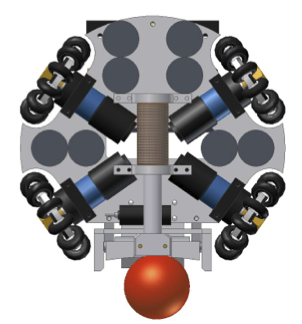
\includegraphics[height=2.5in]{pics/holonomic_robot.png} 
		\caption{\label{robot}Configuration of three groups of motors where $\phi$ is 30, 45, and 60 degrees.}  
 	\end{minipage}
 	\hfill
 	\begin{minipage}[htb]{3in}
		\centering
 		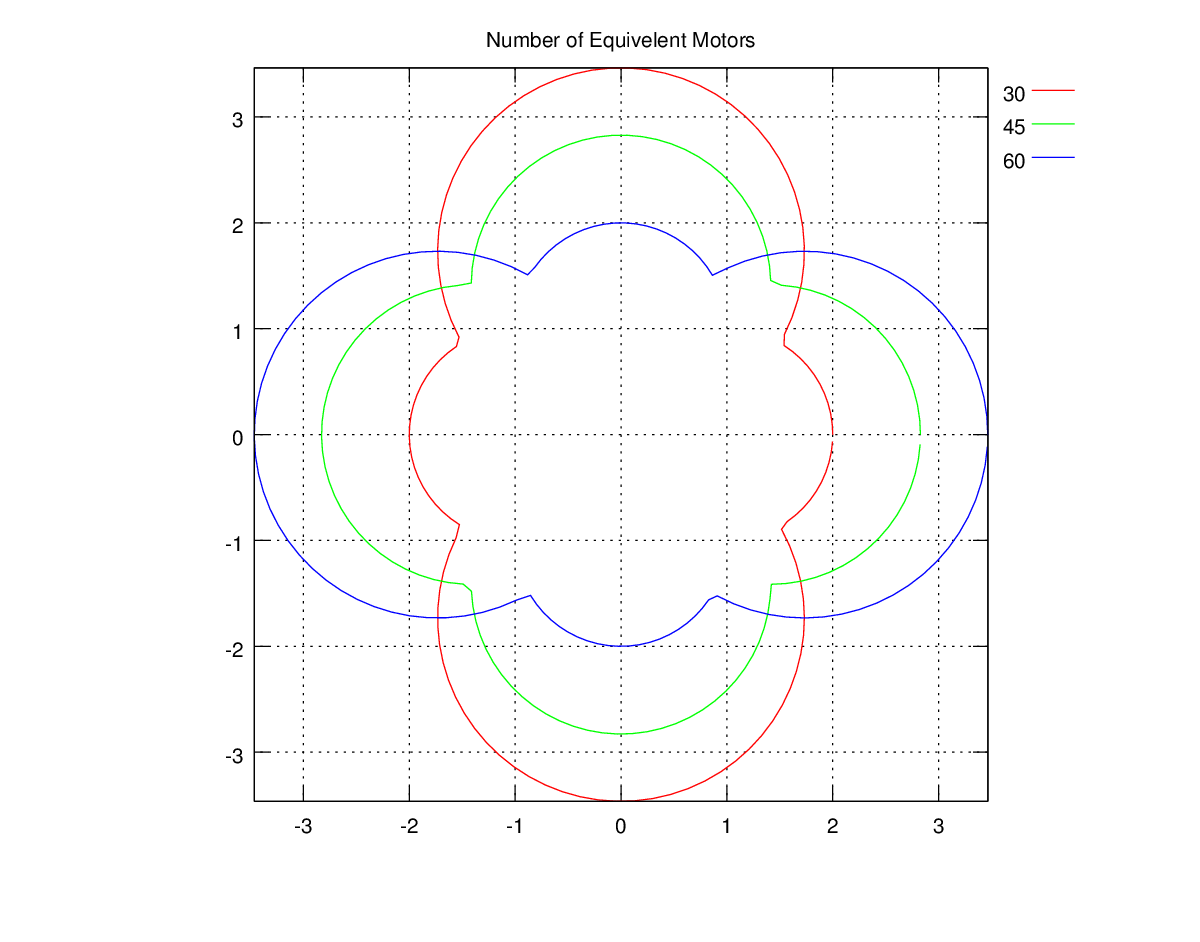
\includegraphics[height =2.5in]{pics/equiv_motors.png} 
		\caption{\label{fig:equivalent_motors} Number of equivalent motors for any direction under linear movement only, no rotational movement allowed.} 
 	\end{minipage} 
\end{figure*}  

Now it is interesting to note that when $\phi$ is set to 30$^\circ$, the robot has more equivalent motors when going forward or backwards, while a $\phi$ of 60$^\circ$ provides more equivalent motors moving left or right. When the motors are are angled at 45$^\circ$, movement is clearly equally optimized for both forward/backwards and left/right ($2 \sin(45)$ is 2.83 motors) movement.

\figref{fig:equivalent_motors} tells us that no mater how the 4 motors are oriented in a realistic configuration, the robot will never have the equivalent use of all 4 motors. Movement in one direction or another can be optimized, but then a sacrifice is made in another direction. This fact is intuitively obvious.

Another issue is these results are also ideal. This logic assumes that the wheels will not slip and have good traction in any orientation. Unfortunately real world results do not mimic this situation and the robot's performance will be reduced.

\section{Control}

Looking at the state space equations, the system is controllable but it is not observable. Using an IMU (accelerometer, gyro, and magnometer), the heading ($\theta$) can be determined from the magnometer and the angular rate ($\omega$) can be determined from the gyro. An observer must be used to estimate the position and velocity of the robot. 

Typically encoders attached to the wheels (under the assumption of no slip) would be used to estimate velocity and position. However, with omni wheels, this is not possible since they rely on slippage in order to achieve holonomic motion. Wheel encoders can be useful for detecting excessive amounts of wheel slippage \cite{Radu} in order to optimize movement or detect failed motors.

\section{Guidance and Navigation}

In order to have the robot go from one location to another, the position and velocity must be estimated. A Kalman filter using the dynamic equations above will provide this solution. The general form of the Kalman filter can be found in any text book on estimation \cite{kf} and have the form:

\begin{eqnarray}
	x=ax+bu \\
	\tilde x = \hat x - x
\end{eqnarray}

where the error ($\tilde x$) is the difference between the estimated state ($\hat x$) and the true state ($x$).

\section{Hardware Setup}

\subsection{Chasis}

\subsection{Electronic Power System}

\begin{figure*}[tb]
	\begin{minipage}[htb]{3in}
		\centering
 		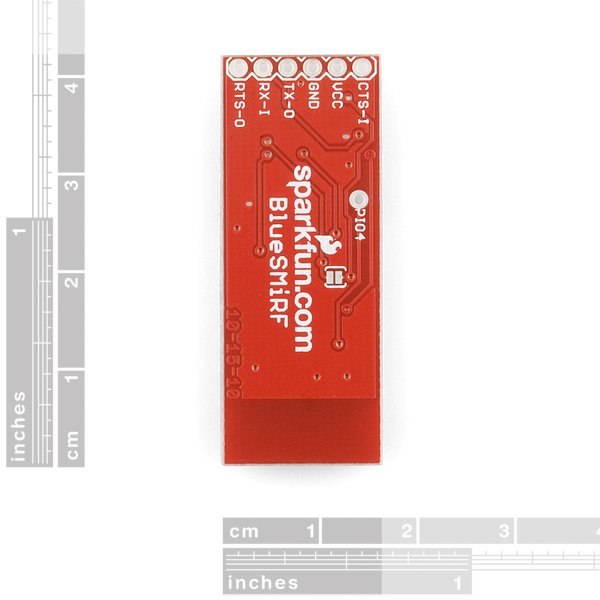
\includegraphics[height=2in]{pics/bluetooth_back.jpg} 
		\caption{\label{fig:imu}IMU.}  
 	\end{minipage}
 	\hfill
 	\begin{minipage}[htb]{3in}
		%\centering
 		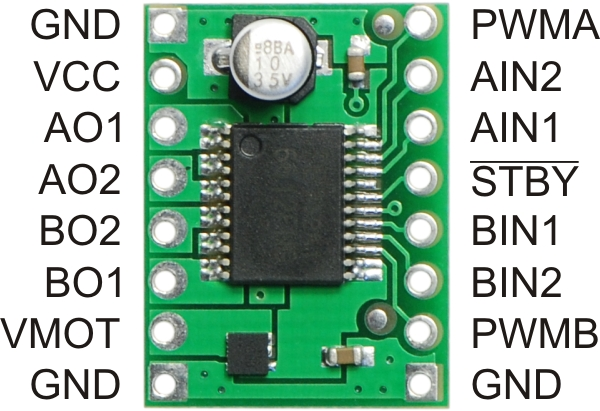
\includegraphics[height =2in]{pics/motor_driver.jpg} 
		%\caption{\label{fig:equivalent_motors} Number of equivalent motors for any direction under linear movement only, no rotational movement allowed.} 
 	\end{minipage} 
\end{figure*}

\subsection{Electronics and Sensors}

\begin{figure*}[tb]
	\begin{minipage}[htb]{3in}
		\centering
 		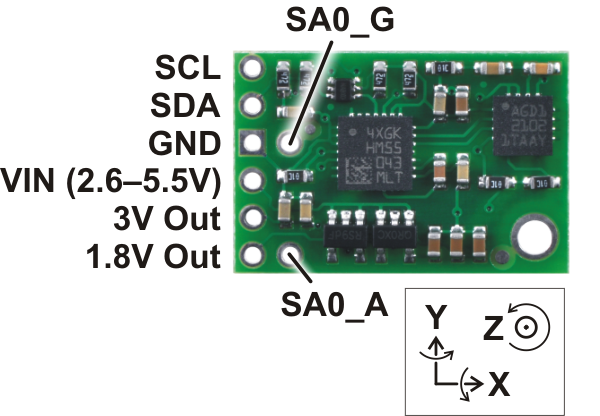
\includegraphics[height=2in]{pics/imu.png} 
		\caption{\label{fig:imu}IMU.}  
 	\end{minipage}
 	\hfill
 	\begin{minipage}[htb]{3in}
		%\centering
 		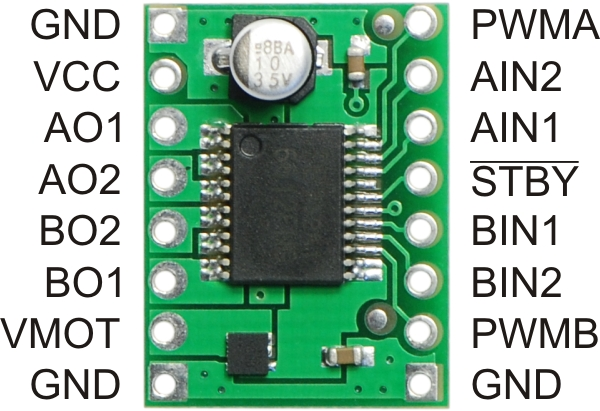
\includegraphics[height =2in]{pics/motor_driver.jpg} 
		%\caption{\label{fig:equivalent_motors} Number of equivalent motors for any direction under linear movement only, no rotational movement allowed.} 
 	\end{minipage} 
\end{figure*}

The robot is teleoperated from a laptop via a bluetooth link to an Arduino microcontroller which runs the motor drivers and sensors.

\subsubsection{MiniIMU}

\subsubsection{Camera}

\subsection{Software}

\begin{figure*}[tb]
	%\begin{minipage}[htb]{3in}
		\centering
 		%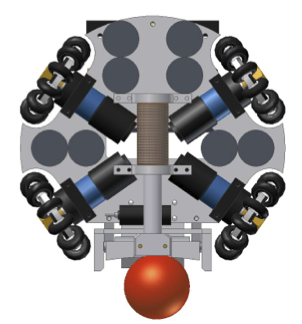
\includegraphics[height=2.5in]{pics/holonomic_robot.png} 
		\caption{\label{fig:ros}The software architecture composed of ROS nodes.}  
 	%\end{minipage}
 	%\hfill
 	%\begin{minipage}[htb]{3in}
		%\centering
 		%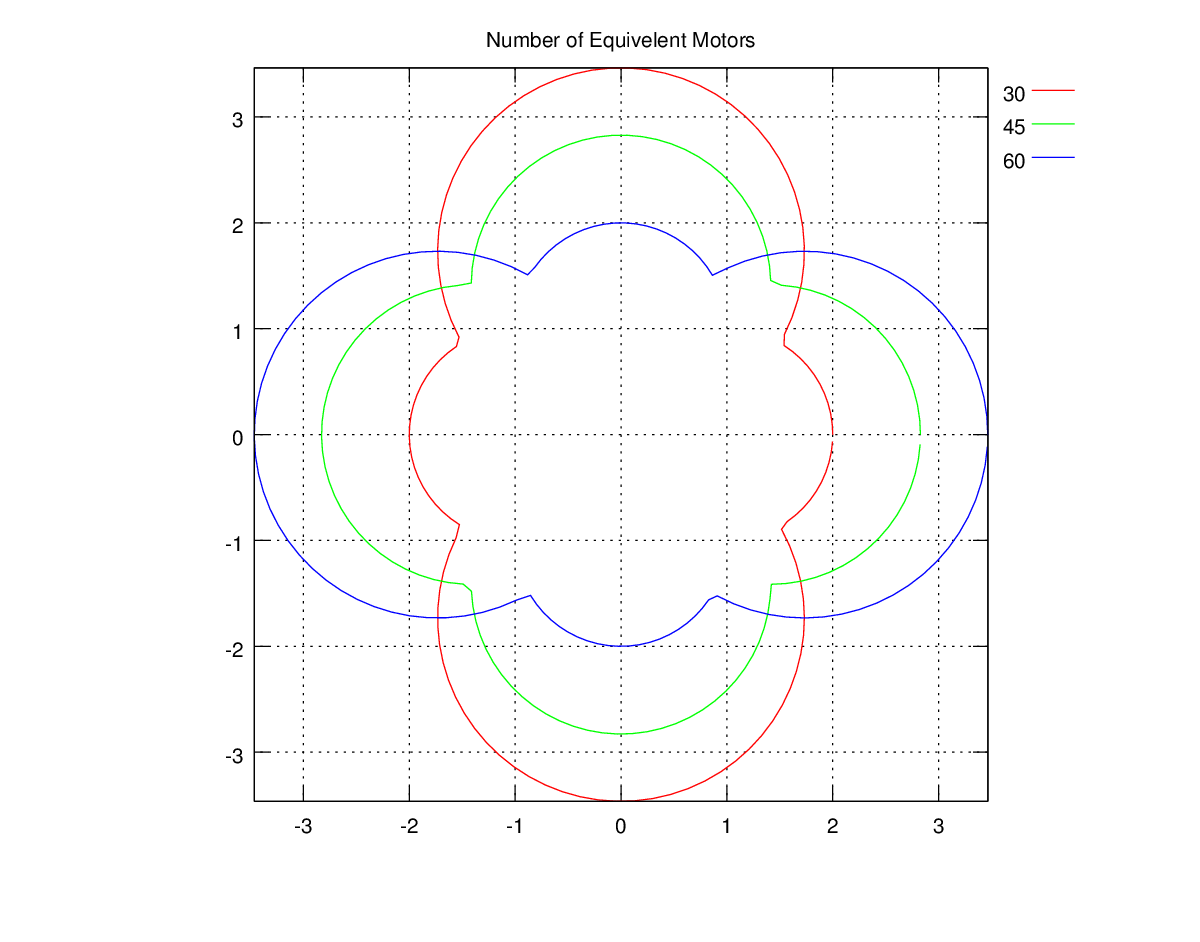
\includegraphics[height =2.5in]{pics/equiv_motors.png} 
		%\caption{\label{fig:equivalent_motors} Number of equivalent motors for any direction under linear movement only, no rotational movement allowed.} 
 	%\end{minipage} 
\end{figure*}
  
The robot utilizes the open source Robotic Operating System (ROS) \cite{ros}. The core software is run on a laptop and commands and telemetry is passed back and forth via serial bluetooth. 

\subsubsection{OpenCV}

The vision system uses the Open Computer Vision (OpenCV \cite{opencv}) to ...

\begin{figure*}[tb]
	\begin{minipage}[htb]{3in}
		\centering
 		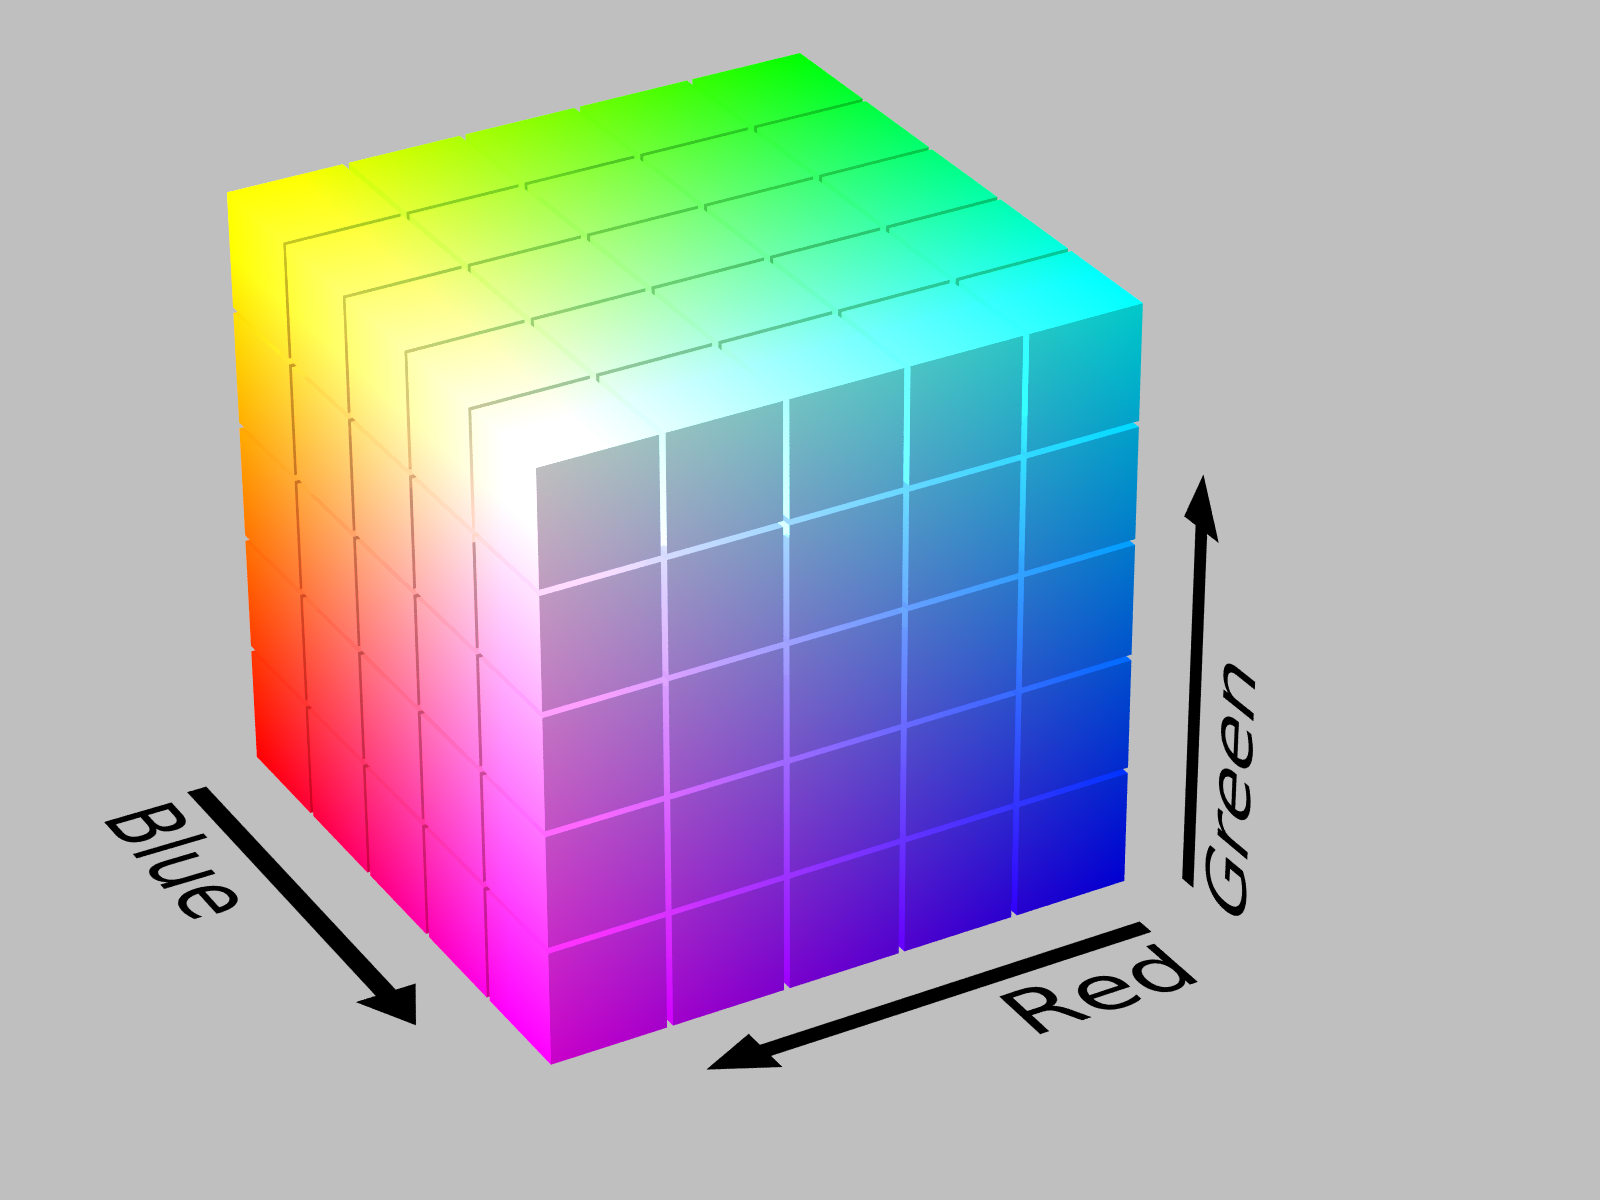
\includegraphics[height=2in]{pics/rgb.png} 
		\caption{\label{fig:rgb}RGB color cube.}  
 	\end{minipage}
 	\hfill
 	\begin{minipage}[htb]{3in}
		\centering
 		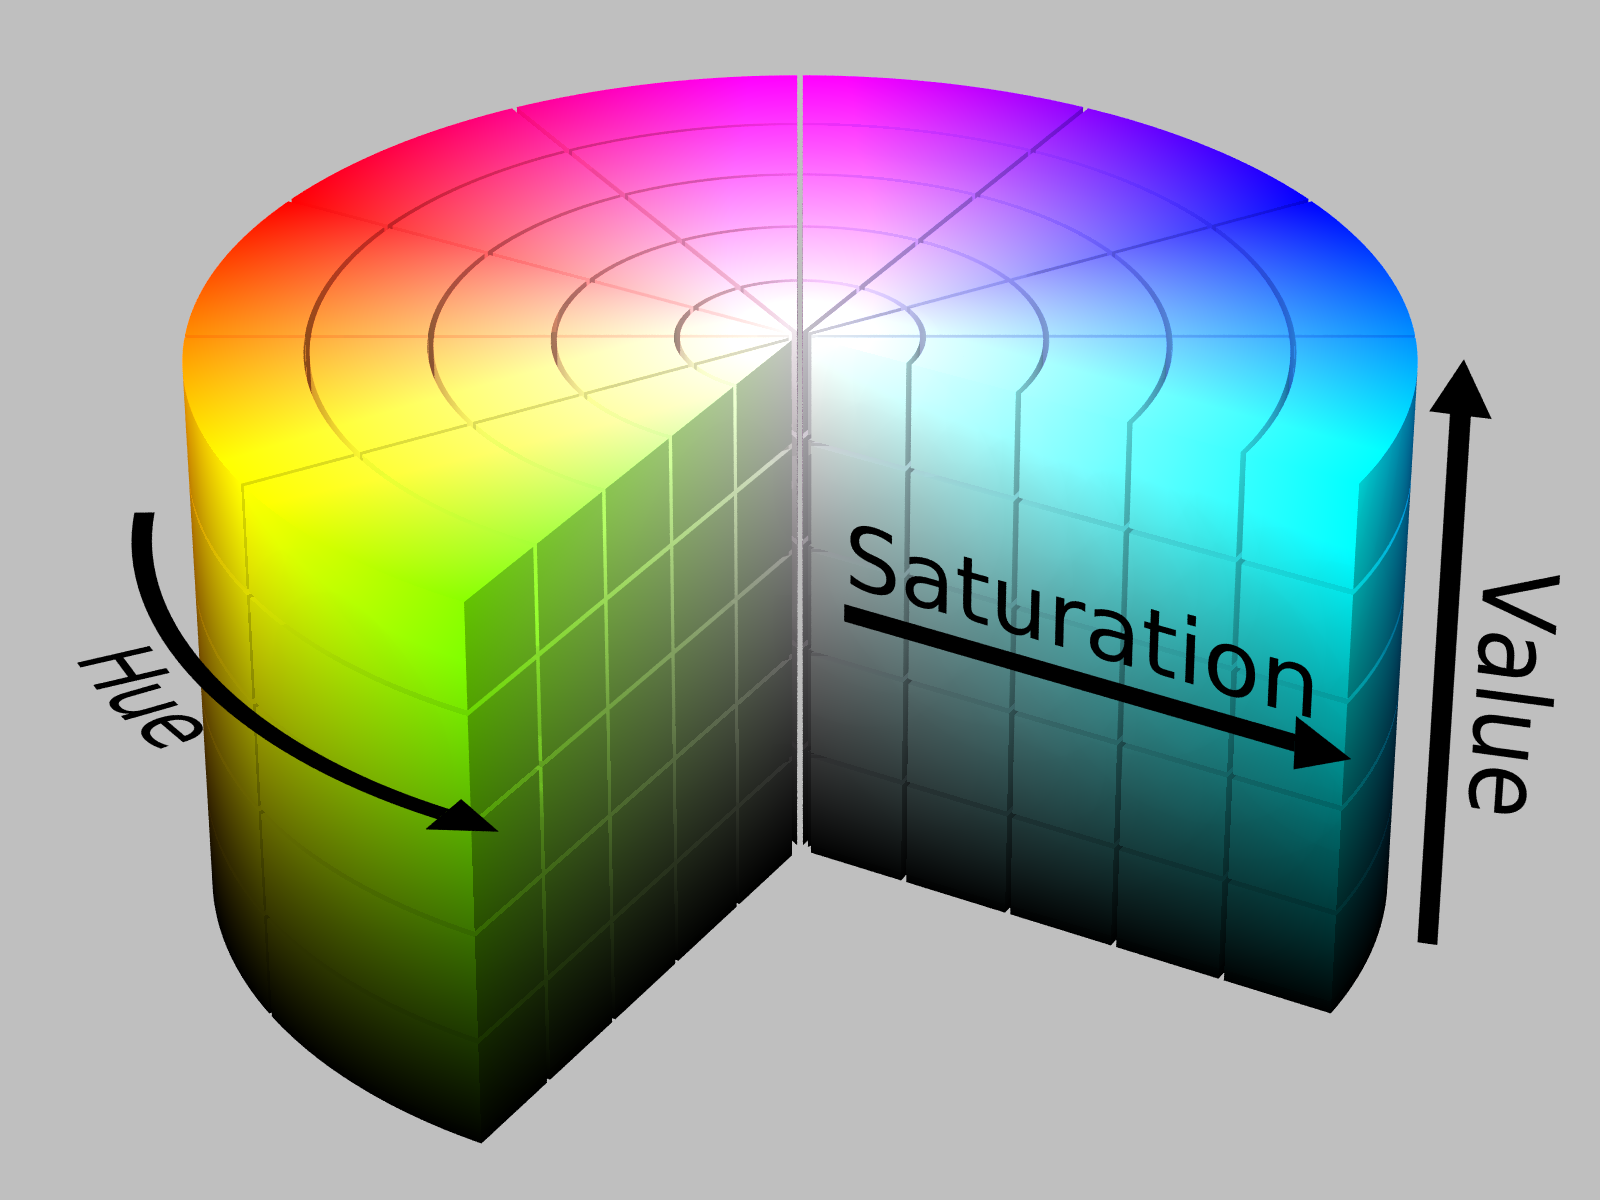
\includegraphics[height =2in]{pics/hsv.png} 
		\caption{\label{fig:hsv} HSV color cylinder.} 
 	\end{minipage} 
\end{figure*}

\begin{description}
	\item[Hue] The "attribute of a visual sensation according to which an area appears to be similar to one of the perceived colors: red, yellow, green, and blue, or to a combination of two of them"
	\item[Saturation] The "colorfulness of a stimulus relative to its own brightness"
	\item[Value, Lightness] The "brightness relative to the brightness of a similarly illuminated white"
\end{description}

\subsubsection{Point Cloud Library}

\section{Results}

\section{References}
\begin{thebibliography}{20}

\bibitem{Radu1} Radu.   

\bibitem{Radu} Radu.   

\bibitem{wheel_slip}
R. Balakrishna, Ashitava Ghosal, "Modeling of Slip for Wheeled Mobile Robots," lEEE TRANSACTIONS ON ROBOTICS AND AUTOMATION, VOL. I I , NO. I , FEBRUARY 1995, pp. 126-132

\bibitem{wheel_slip2} J. Agullo, S. Cardona, and J. Vivancos, �Kinematics of vehicles with directional sliding wheels,� Mechanisms and Muchine Theory, vol. 22, no. 4, pp. 295-301, 1987.

\bibitem{ros} \url{http://www.ros.org}

\bibitem{color_space} \url{http://en.wikipedia.org/wiki/HSL_and_HSV}

\bibitem{pcl} \url{http://pointclouds.org}

\bibitem{opencv} \url{http://opencv.willowgarage.com}

\bibitem{wiki_non_holonomic} \url{http://en.wikipedia.org/wiki/Non-holonomic_system}

\bibitem{wiki_lagrange} \url{http://en.wikipedia.org/wiki/Lagrangian_mechanics}

\bibitem{kf} kalman filter

\end{thebibliography}


\end{document}